
%%% Local Variables: 
%%% mode: latex
%%% TeX-master: "main"
%%% End: 
\section{Initial Assembly}

% This section should highlight the comparison between the full-data assembly and that conducted with only the properly paired reads.
% It should emphasize the larger number of ORFs recapitulated by the properly paired reads, and the improved mappability of such a dataset.
% Therefore, at the cost of lower effective sequencing depth, transcripts from the properly paired dataset are less likely to be false positives resulting from the low mappability of improper pairs.
Initial transcriptome assemblies were conducted for the full dataset and the subset of properly-paired reads. Both assemblies were compared to address questions regarding assembly performance (Table \ref{table:assemb_compare}). Would extra improperly-paired or unpaired reads improve the precision of boundary estimates, potentially as terminal or bridging reads? Alternatively, the properly-paired subset could have resulted in a simpler and cleaner graph for traversal by the assembly algorithm. Both of the resulting assemblies were compared by their qualities, such as assembly size, transcript lengths, and inclusion of the reference protein annotations. 

In this comparison, the assemblies were inspected for errors that affect these qualities. The previous chapter described techniques for the minimization of frequently ignored background signals, not quantified by similar studies. While spectrophotometric and electrophoretic analyses suggested pure RNA, some residual signals are often encountered in RNA-seq studies.\cite{176} Automated methods such as assembly encounter difficulty when background and overlapping signals are sufficiently complex. To identify potential false positives, the results were inspected for misassemblies, artifacts from the graphs constructed for the dataset. Documentation and analysis of these artifacts was required for assembly selection.

\begin{table}
\caption{Assembly Comparison}\label{table:assemb_compare}
\begin{center}
\begin{tabular}{|c|c|c|}\hline
  & All Reads & Proper Pairs\\\hline\hline
Transcripts & 3054 & 4295\\\hline
Sequenced Mb & 6.1 & 7.2\\\hline
Length Range & 200-28kb & 200-35kb\\\hline
ORFs & 2397 (63\%) & 3225 (85\%)\\\hline
Standard Transcripts & 796 (27\%) & 1029 (24\%)\\\hline
Standard Mb & 3.7 (61\%) & 4.56 (63\%)\\\hline
Novel Transcripts & 2129 (73\%) & 3266 (76\%)\\\hline
Novel Mb & 2.4 (39\%)& 2.64 (37\%)\\\hline
\end{tabular}
\end{center}
\small
This table contains statistics for the two transcriptome assemblies, the first with all sequenced reads and the second with only proper-pairs. The total number of assembled transcripts and the size of their span is reported. The number and percentage of reference ORFs contained within the so called ``standard'' transcripts is provided. Additionally, the number of the standard transcripts and their span is provided additionally. The same statistics are presented for novel transcripts as well.
\end{table}

\subsubsection{Assembly Comparison}
First, simple statistics were compiled for both assemblies (Table \ref{table:assemb_compare}). The transcripts that contained reference protein annotations (referred to as ``standard'' transcripts), were approximately 25\% by number of assembled transcripts, yet they accounted for 63\% of the assembled basepairs for both datasets. Upon inspection, the assembly from the subset of properly-paired reads was larger and more inclusive, recalling 85\% of the reference ORFs. Also, this assembly had higher per-base sequencing depth in both ``standard'' and ``novel'' transcripts (\ref{fig:5.1}). While the transcript lengths were comparable (\ref{fig:5.2a}), the assembly from all reads had lower expression, size, and inclusiveness of the reference CDSes compared to the subset. Therefore, the transcript coordinates from the uncurated properly-paired assembly were used for further analysis of feature length, UTR length, and expression.




\begin{figure}
\small
\begin{center}
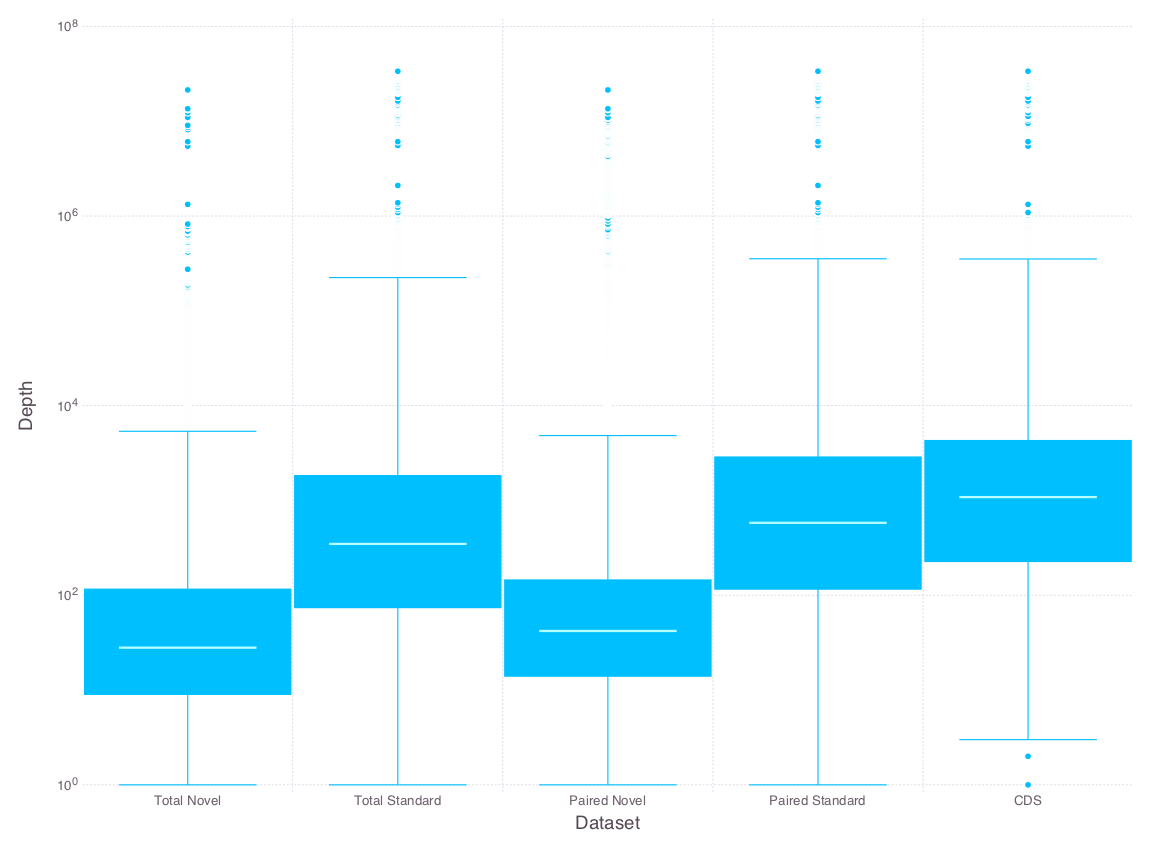
\includegraphics[width=\textwidth,height=4in]{images/Assembly/Comparison/PairvsTot_boxplot.png}
\end{center}
\caption{Transcript Depth Comparison}\label{fig:5.1}
\end{figure}


\begin{figure}[t]
\small
\begin{center}
\begin{minipage}{.5\textwidth}
\begin{center}
{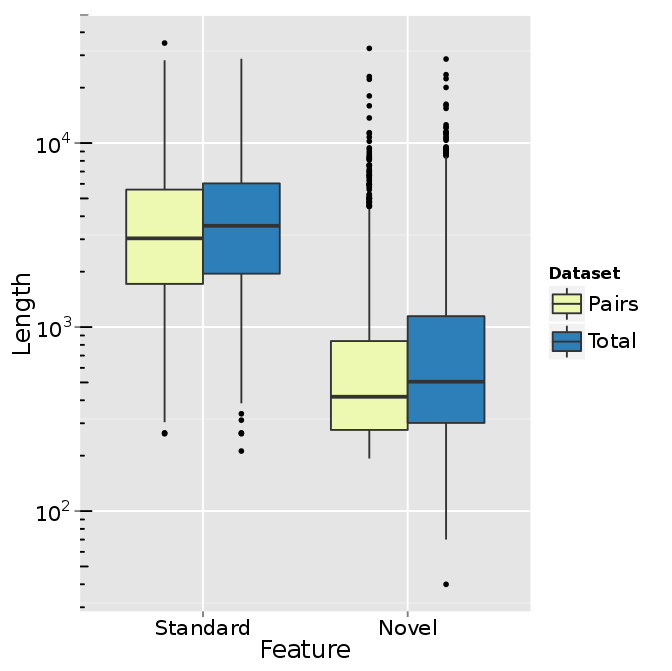
\includegraphics[width=\linewidth,height=2.5in]{images/Assembly/Comparison/TotvsPaired_length.png}
\subcaption{Length Comparison}\label{fig:5.2a}}
\end{center}
\end{minipage}%
\begin{minipage}{.5\textwidth}
\begin{center}
{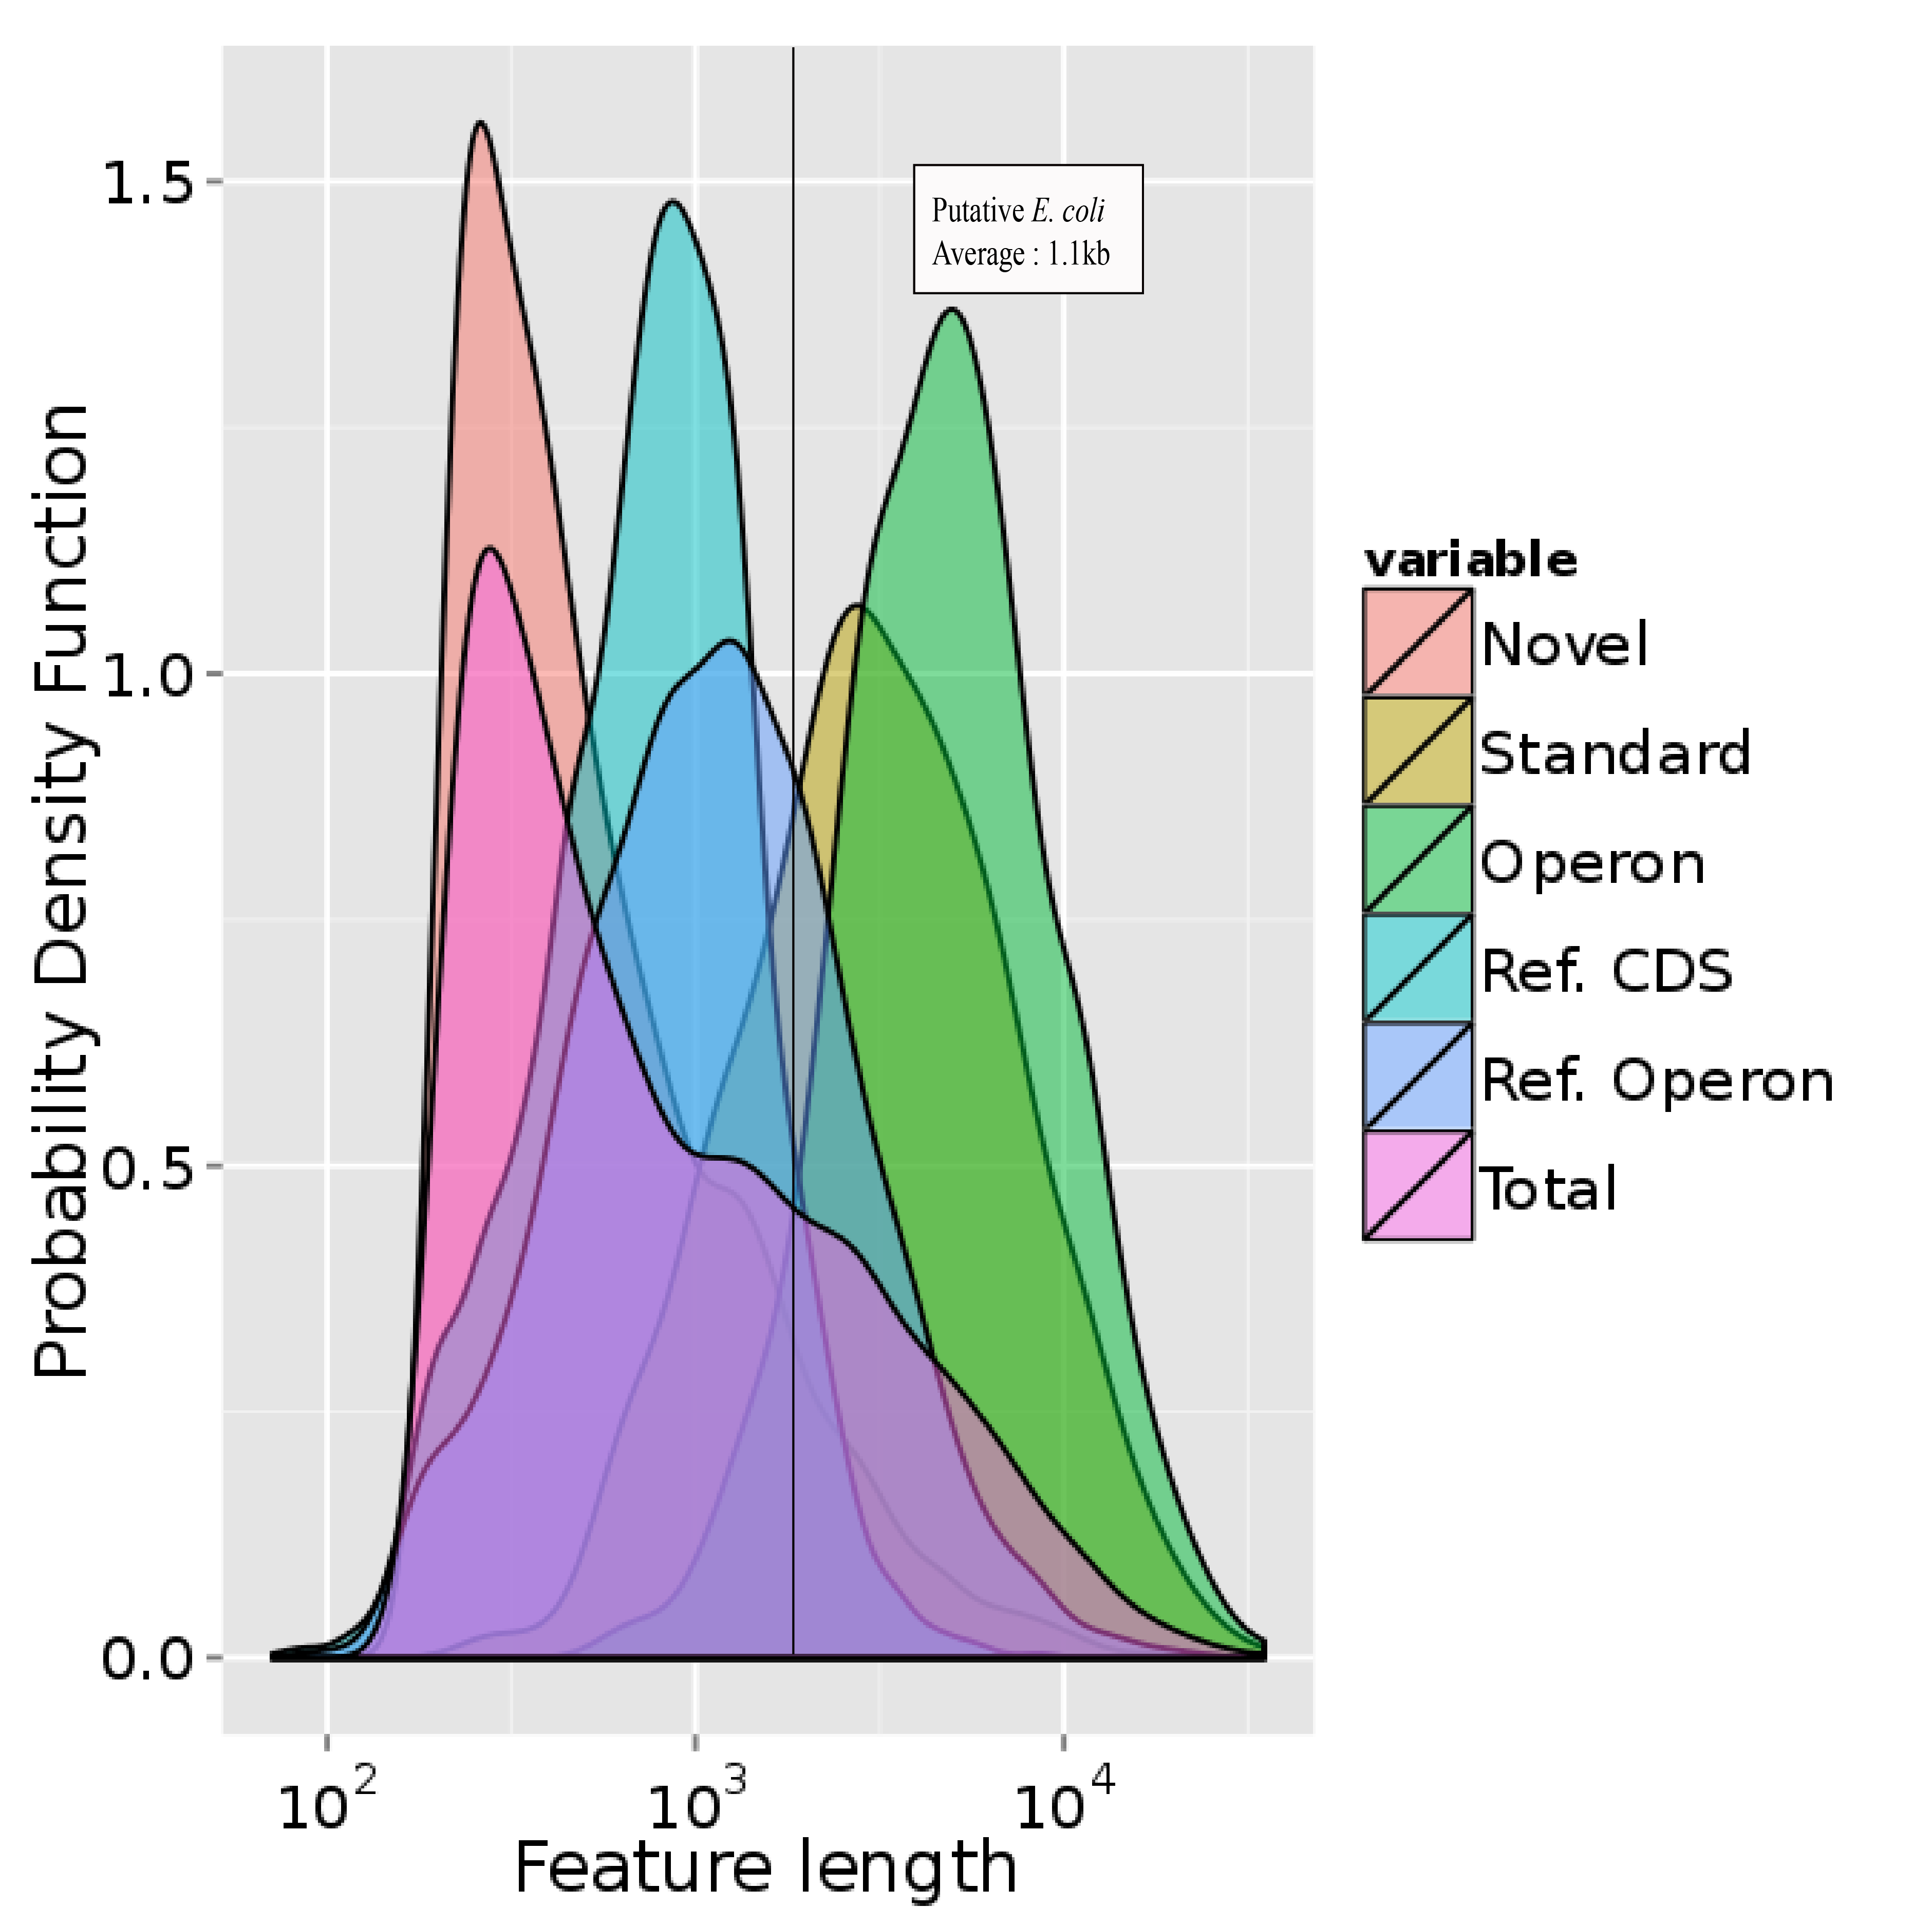
\includegraphics[width=\linewidth,height=2.5in]{images/Assembly/Summary/ffeature_length_1.png}
\subcaption{Feature Lengths}\label{fig:5.2b}}
\end{center}
\end{minipage}
\end{center}
\caption{Transcript Length Comparison and Uncurated Feature Lengths}
With improved inclusiveness (Table \ref{table:assemb_compare}), expression levels(Figure \ref{fig:5.1}), and comparable transcript sizes \subref{fig:5.2a}), the uncurated assembly from the properly-paired reads was selected for further evaluation. \subref{fig:5.2b}) ``Standard'' transcripts, both mono and polycistronic (operon), are present along with 3120 putative novel transcripts. The standard transcripts are close in size to prokaryotic norms\cite{86}.
\end{figure}


\subsubsection{Uncurated Assembly Statistics}

In the uncurated assembly, 4,177 transcripts spanning 7.18Mb were assembled. This size is 88\% of the maximum possible size in \textit{C. acetobutylicum}. Each transcript aligned to a single location in the genome with \textgreater 98\% identity and less than 30bp of gaps, suggesting high quality assembly results. Of these, 1,029 standard transcripts spanning 4.56Mb contained 3,225(86\%) reference protein annotations. The remaining 3,120 (75\% by number, 36.5\% by basepairs) were potentially novel transcripts, lengths ranging from 200-32.7kb. These whole-transcriptome statistics suggest that the \textit{C. acetobutylicum} transcriptome is large and complex, in agreement with previous findings(keerthi BMC).

\begin{figure}[h!]
\small
\begin{center}
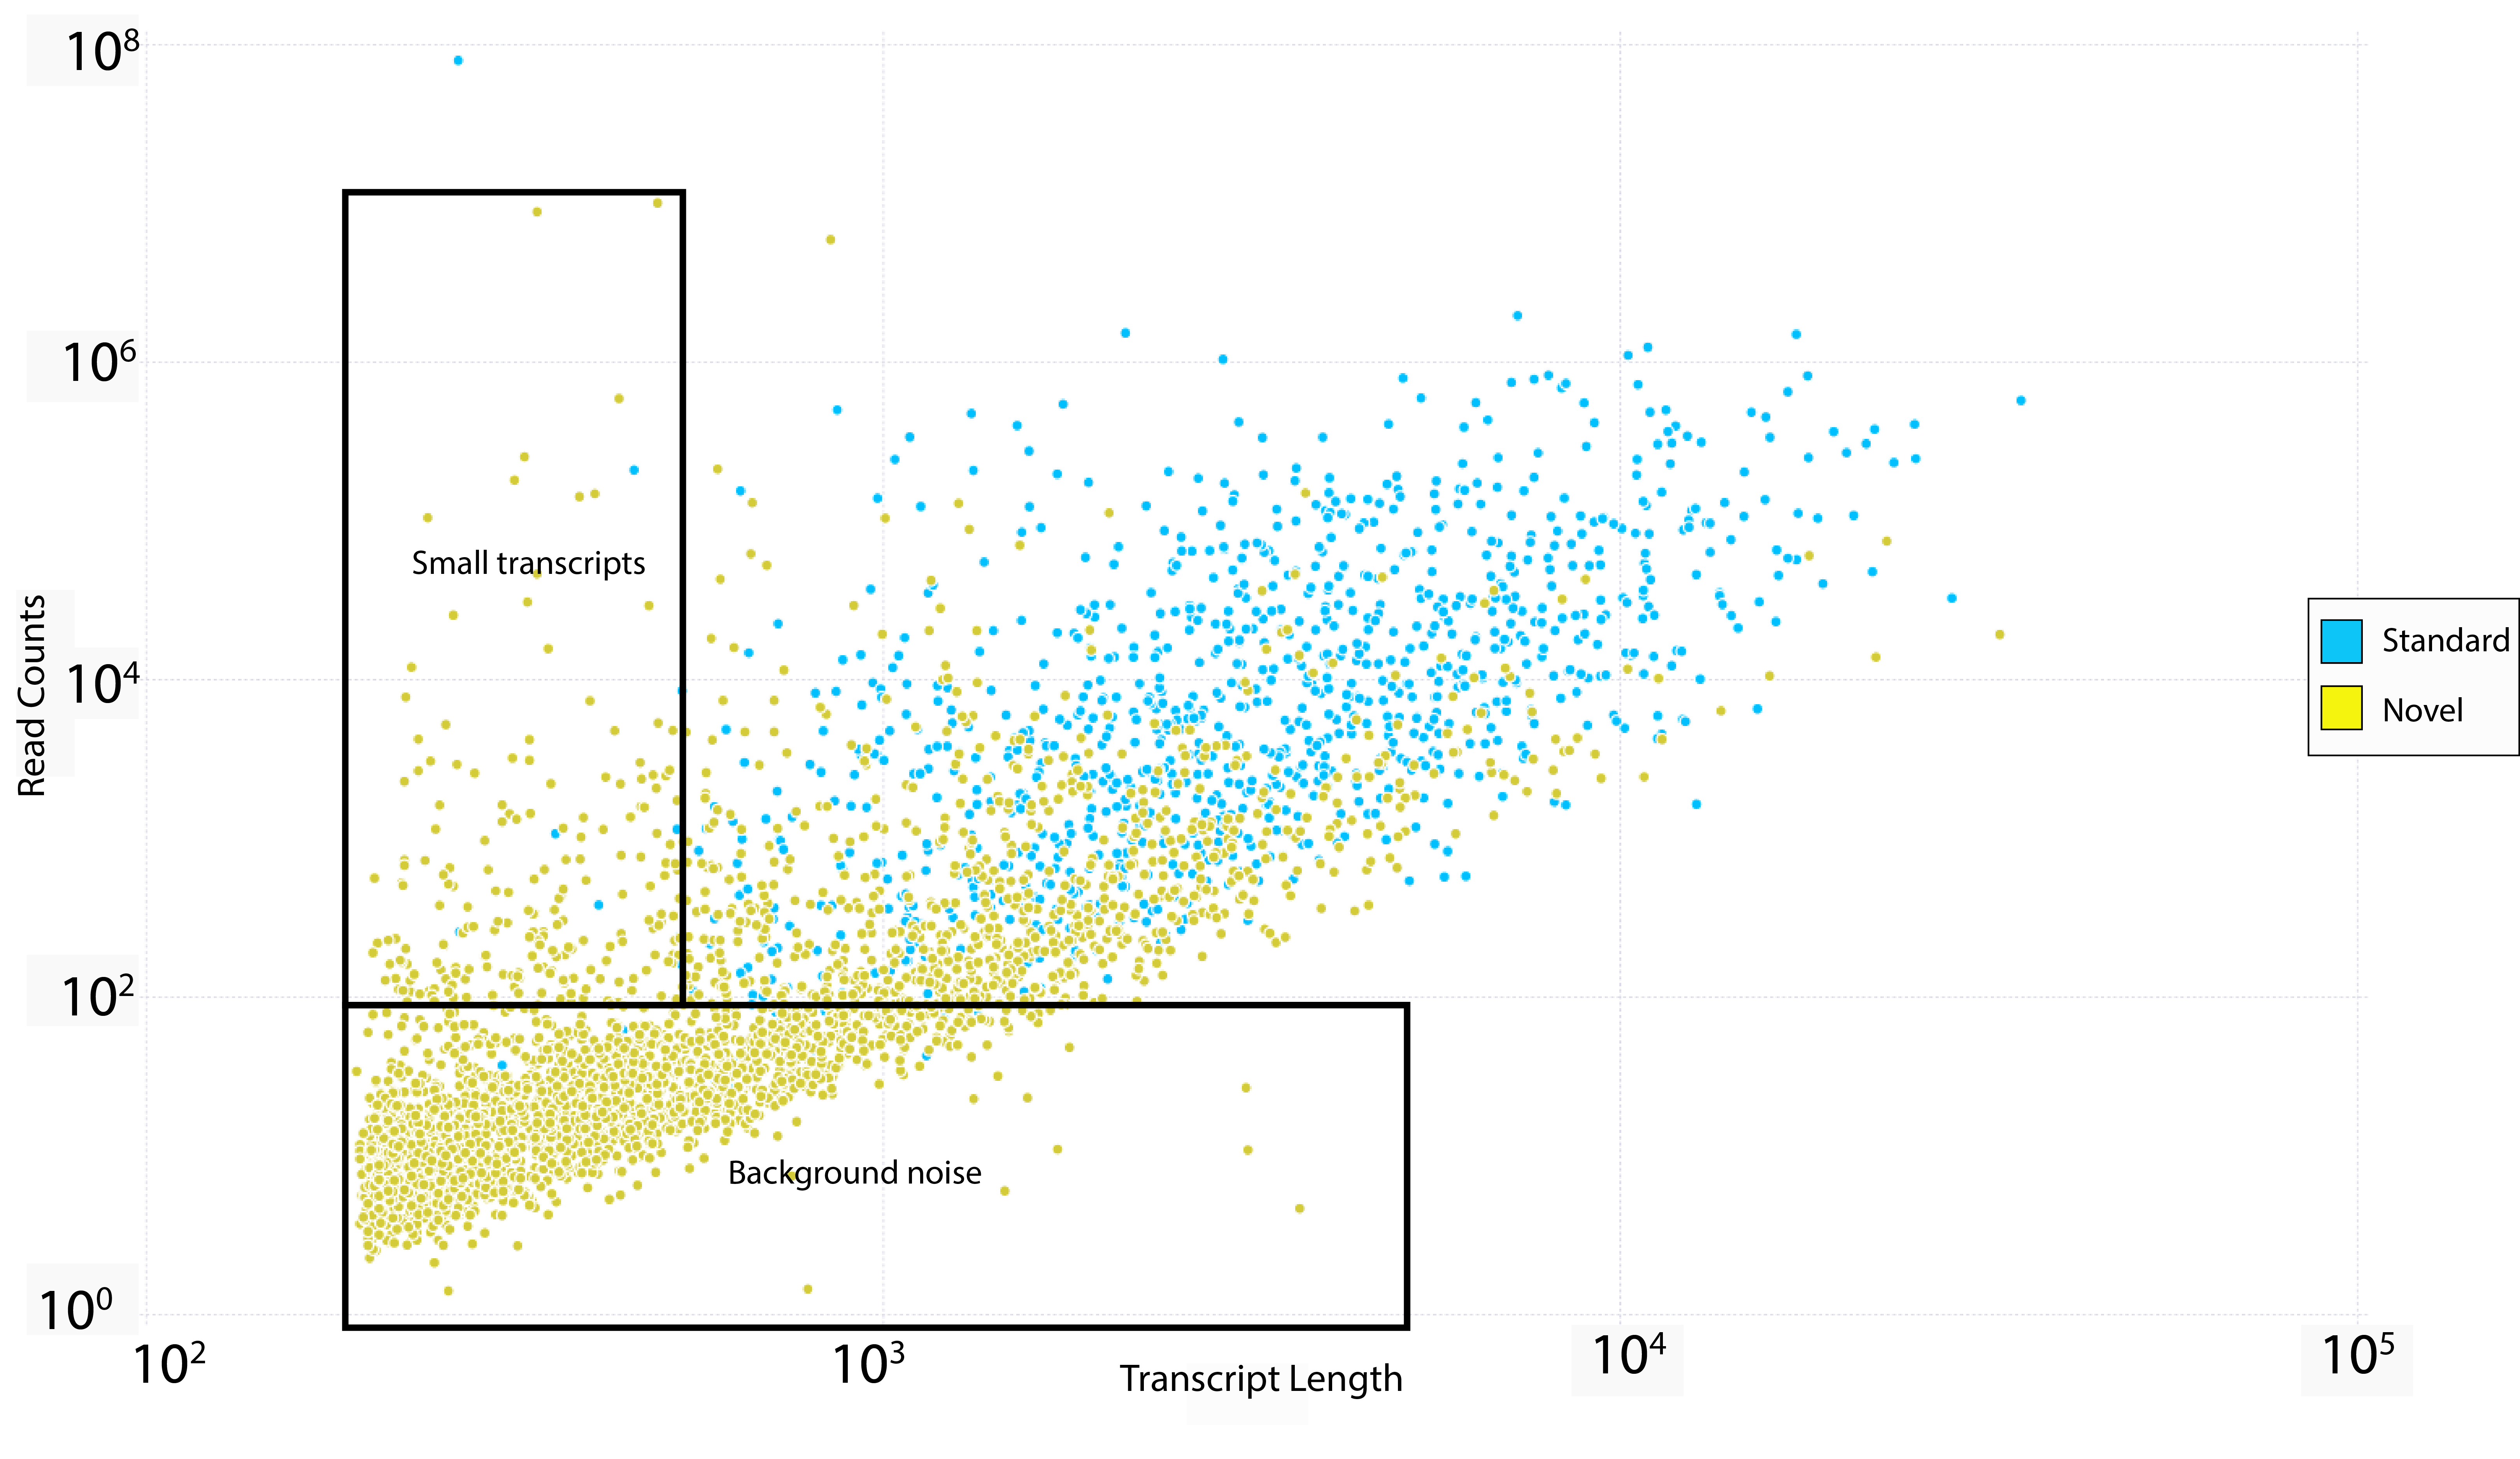
\includegraphics[width=\textwidth,height=4in]{images/Assembly/Summary/Depth_vs_length.png}
\end{center}
\caption{Expression (Avg. Read Count) vs Transcript Length}\label{fig:5.3}
Three additional populations are present in the assembled transcripts. Short novel transcripts with high expression are candidates for \textit{cis}-encoded antisense small RNAs. Those that are long in length with weaker expression tend to be found antisense from a standard transcript and thus represent background antisense signal (\textless 5\% sense expression). However, the majority of the novel transcripts are short in length with weak transcription and most likely represent background signals such as spurious transcription.
\end{figure}

Additional data showed the characteristics of the transcripts themselves and painted a complicated picture. The standard transcripts, including mono and poly-cistronic transcripts, were larger than the novel set(\ref{fig:5.2b}). More surprisingly, they were larger on average than estimates of the mean transcript size in \textit{E. coli}\cite{86}. In addition, the standard set possessed higher levels of expression(\ref{fig:5.1}). Together, there was a trend between length and expression that divided the novel transcripts into distinct classes(\ref{fig:5.3}). The majority of the novel transcripts were short in length (200-500bp) with low read counts. Depending on local depth and annotation patterns, some of these putative transcripts were likely technical artifacts. Longer novel transcripts with similarly low read counts were most likely assemblies of background (1-5\%) or antisense signal. Outside of these groups, there were a number of highly expressed, short, novel transcripts that could reflect small peptide encoding transcripts or small RNAs. Equally expressed and larger transcripts could also represent novel transcripts and protein encoding genes. The trend between transcript length and expression indicated the presence of both novel transcripts and technical artifacts in the assembly results, suggesting that further investigation and correction would be necessary.


\begin{figure}
\small
\begin{center}
\begin{minipage}{.5\textwidth}
\begin{center}
{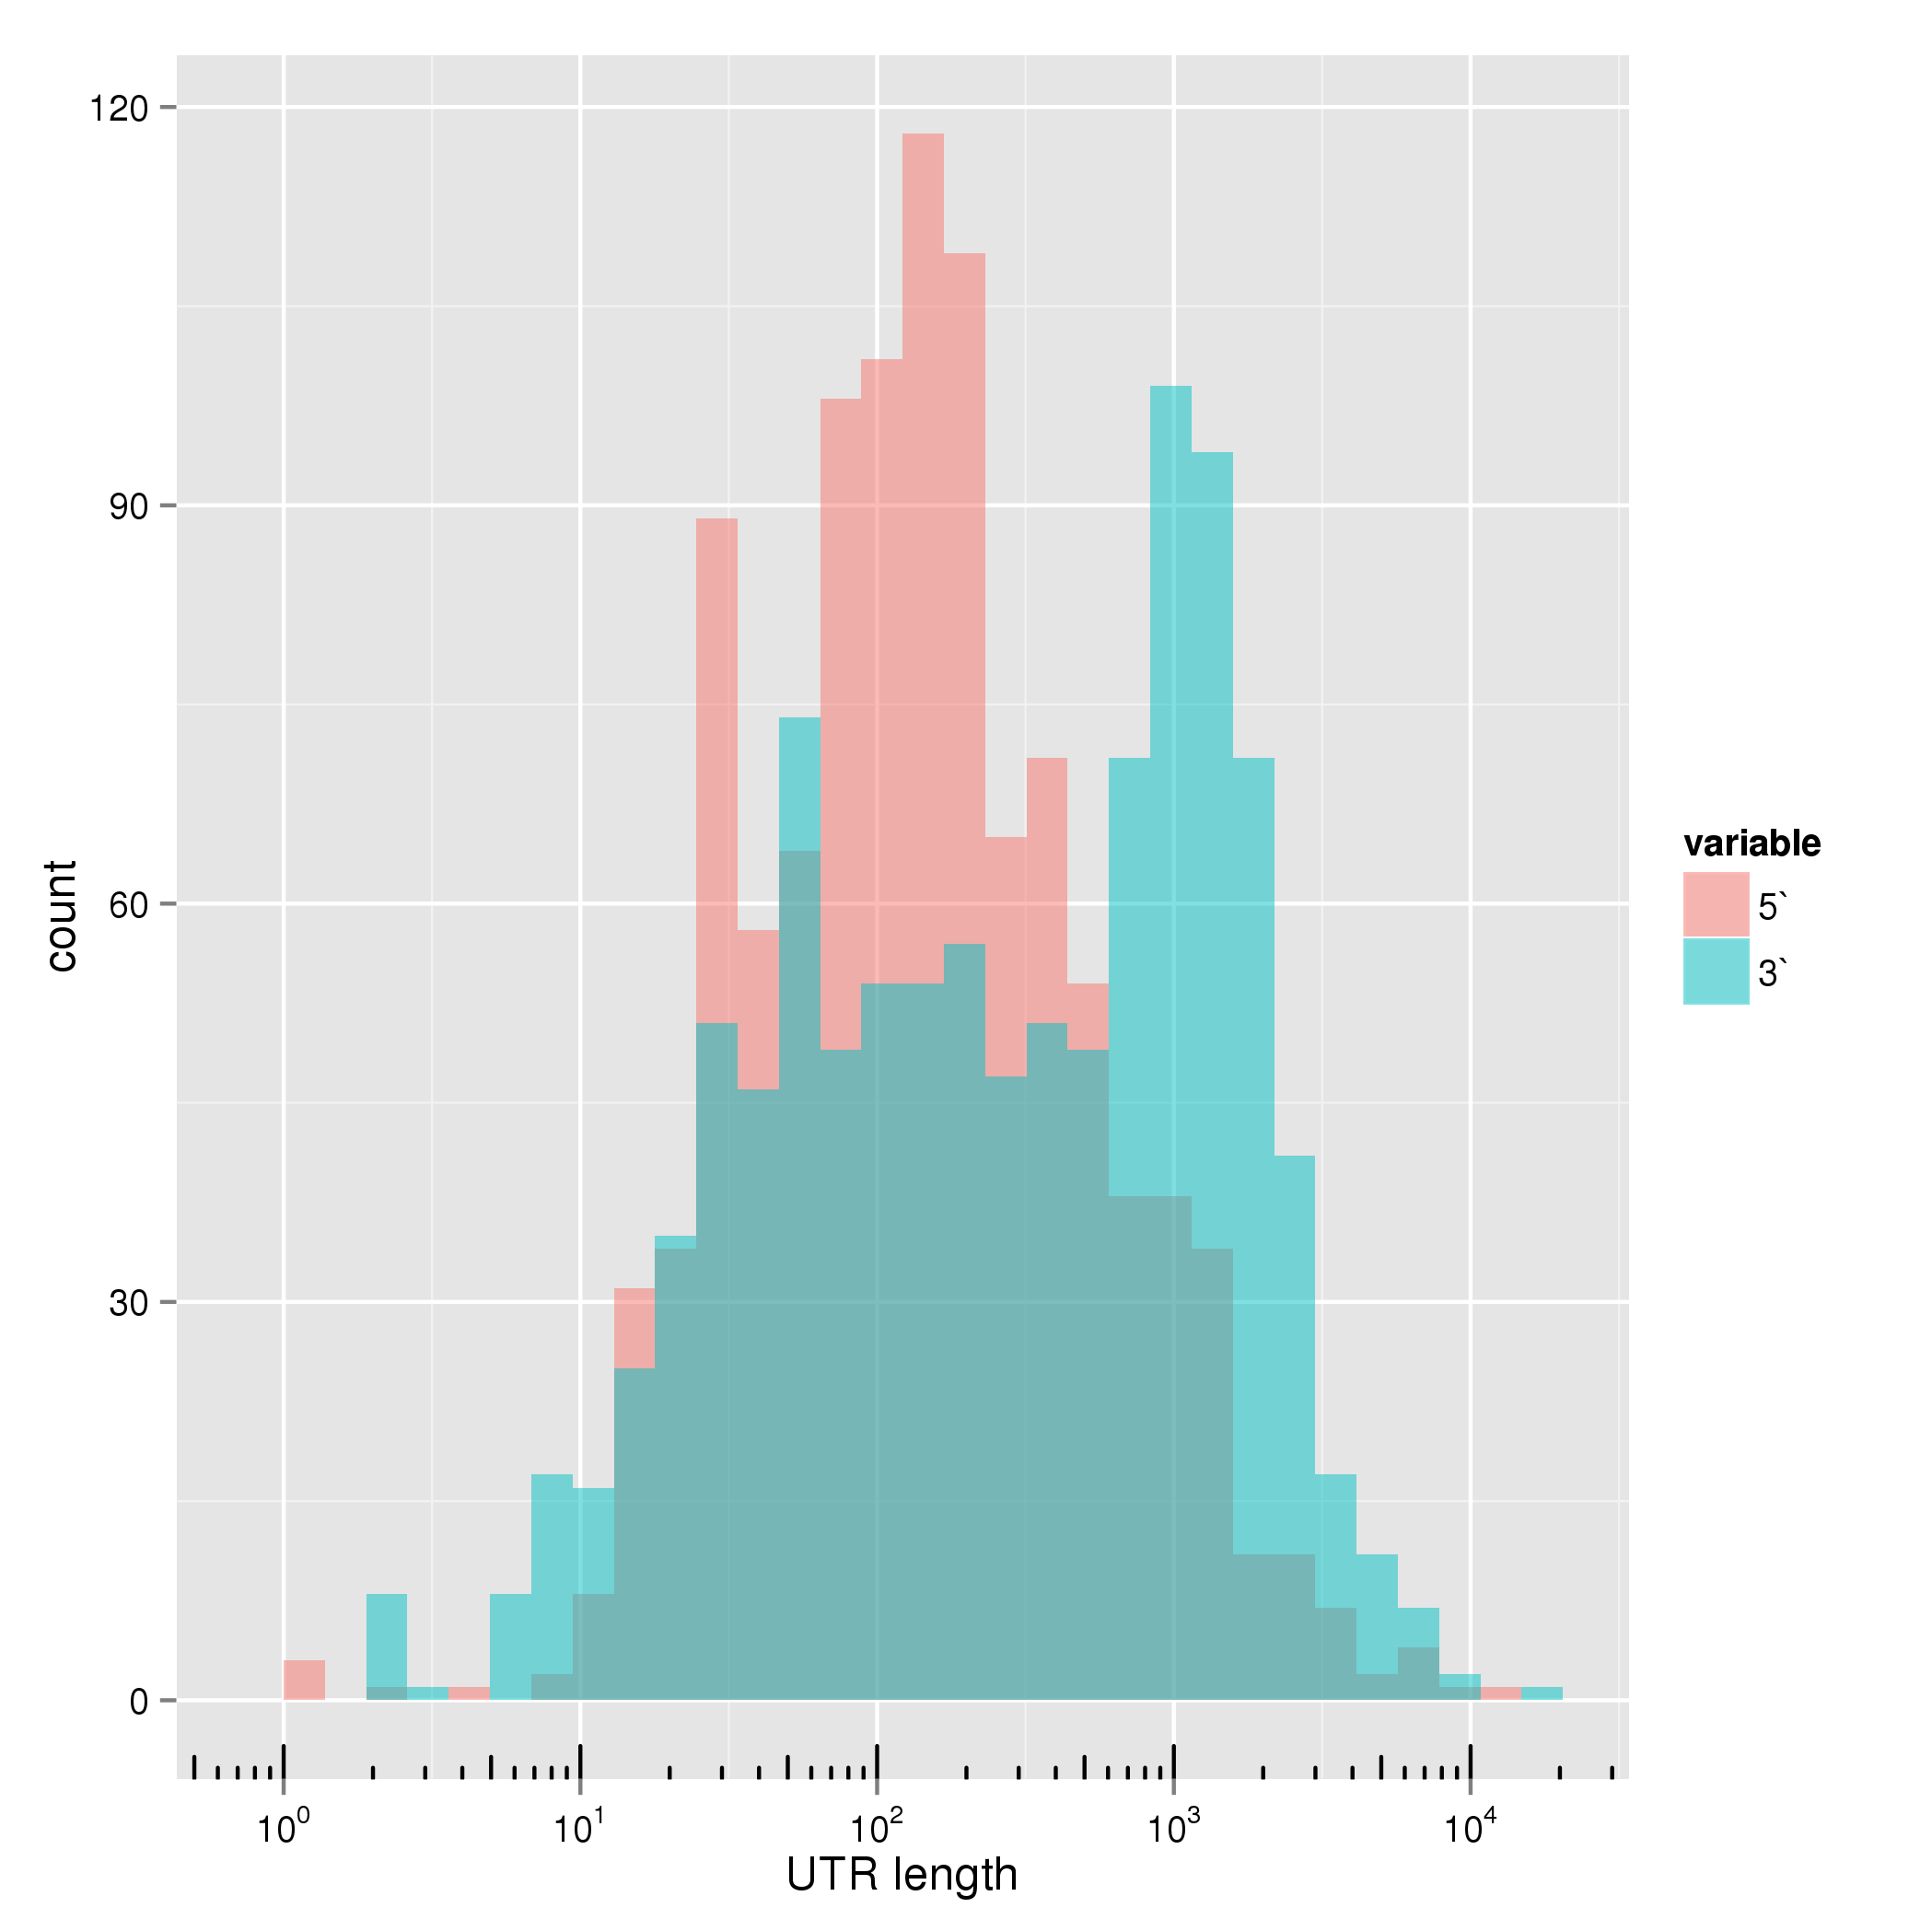
\includegraphics[width=\linewidth,height=3in]{images/Assembly/Summary/futrlength.png}
\subcaption{5' and 3' Untranslated Regions}\label{fig:5.4a}}
\end{center}
\end{minipage}%
\begin{minipage}{.5\textwidth}
\begin{center}
{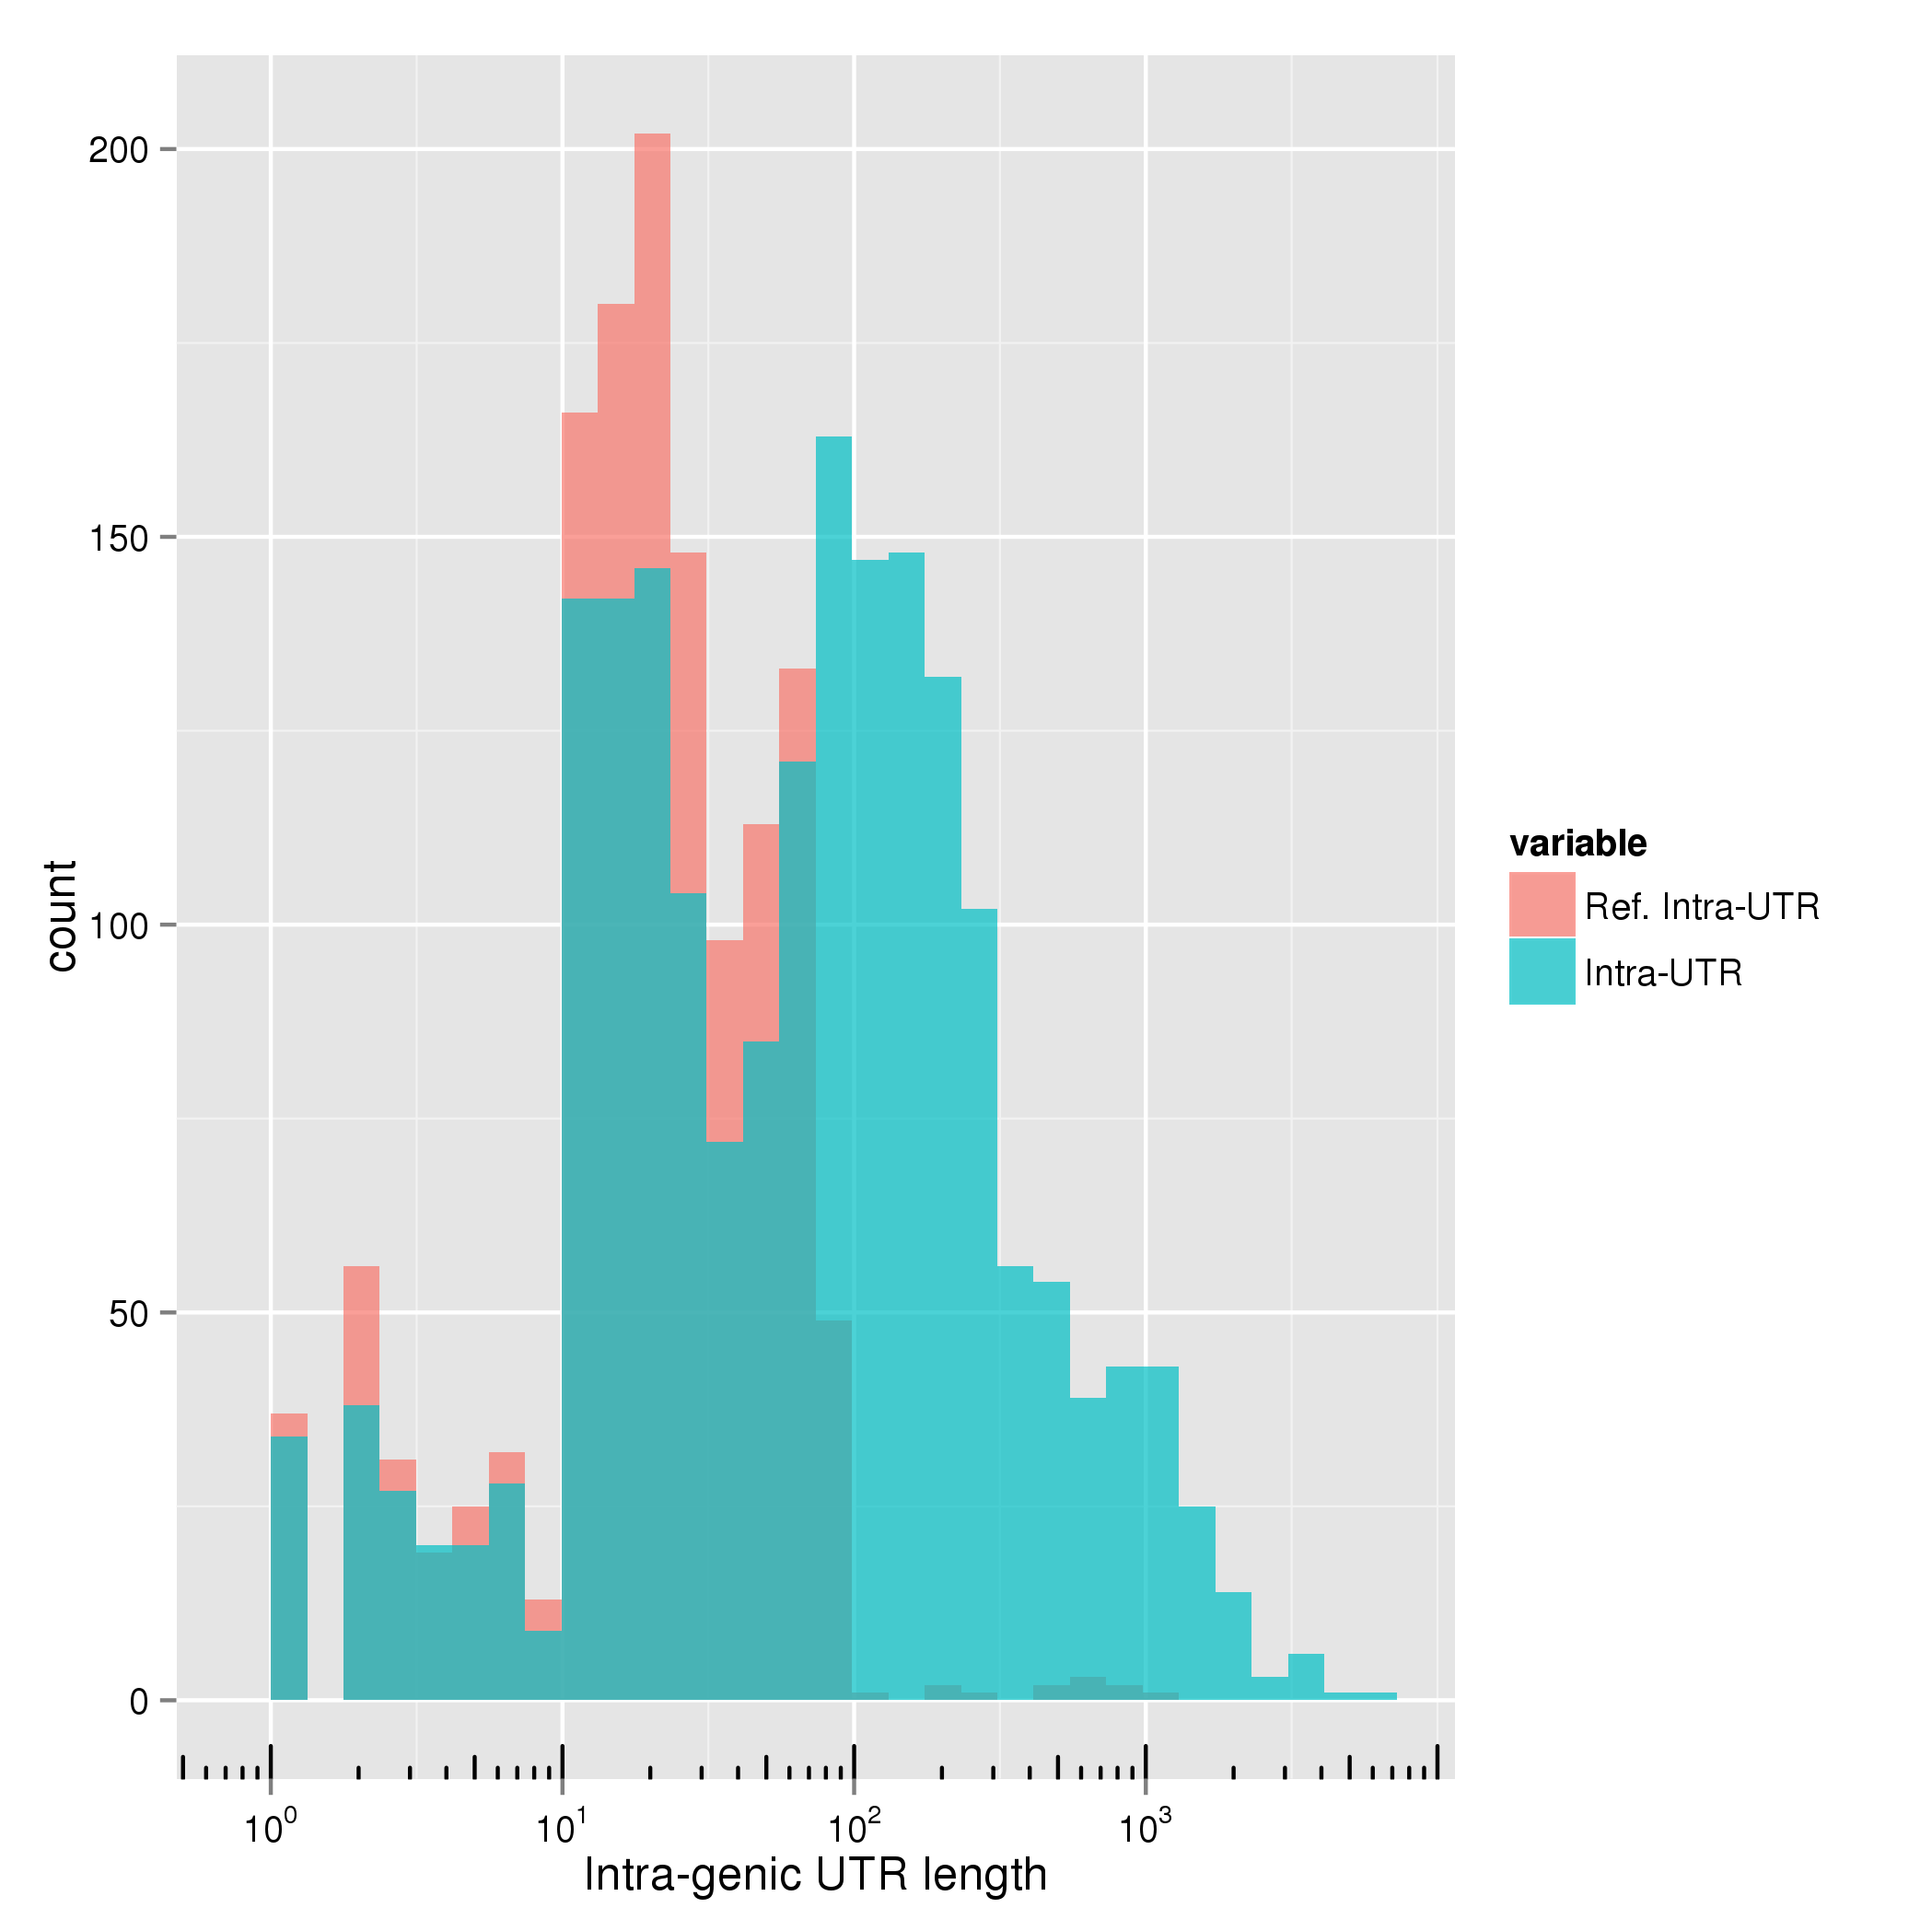
\includegraphics[width=\linewidth,height=3in]{images/Assembly/Summary/fintrautrlength_1.png}
\subcaption{Intra-operonic Untranslated Region}\label{fig:5.4b}}
\end{center}
\end{minipage}
\end{center}
\caption{Untranslated Regions}
The standard transcripts contain untranslated regions that suggest a level of misassembly, indicated by extended 5' and 3' UTRs (\subref{fig:5.4a}). The 3' UTRs display a slightly bimodal pattern. Some of the extended UTRs may encode previously unannotated proteins or riboregulatory elements.
\end{figure}

An additional illustration of misassembly was seen in the distribution of untranslated region (UTR) lengths (\ref{fig:5.4a}). A number of the standard transcripts possess 5' and 3' UTRs that were several hundreds of basepairs in length, while most UTRs previously determined in \textit{C. acetobutylicum}\cite{63,64,69,74,76} and \textit{E. coli}\cite{87} are approximately 100bp. Some of these could have contained riboswitches or unannotated proteins, although likely not at the frequency shown by this histogram. Therefore, it was desirable to address these misassemblies through a curation process.

Nevertheless, encouraging results were obtained from examination of the uncurated assembly of the properly paired reads. This subset produced a large number of transcripts spanning 88\% of the bases of the genome and contained the majority of the reference protein annotations. The large number of assembled basepairs suggested both sufficiently high sensitivity (low false negative rate)and good k-mer complexity in the data. This truly diverse library was likely to contain rare and novel transcripts. Analysis of the novel transcript size and expression suggests that small RNAs and larger protein-encoding messages have been acquired in this dataset in addition to technical artifacts. As expected, false positive transcripts were assembled from background antisense signal or spurious transcription. Additional evidence for these background signals were apparent in large UTR lengths of the standard transcripts. After seeing evidence of these issues in both standard and novel transcripts, it was desirable to closely examine and illustrate these examples. To investigate these issues, a customized genome browser was developed as a tool for curation to increase the precision and accuracy of the transcript coordinates. The integrated curation method involving this tool is discussed next.









